% This version of CVPR template is provided by Ming-Ming Cheng.
% Please leave an issue if you found a bug:
% https://github.com/MCG-NKU/CVPR_Template.

\documentclass[final]{cvpr}

\usepackage{times}
\usepackage{epsfig}
\usepackage{graphicx}
\usepackage{amsmath}
\usepackage{amssymb}

% Include other packages here, before hyperref.
\usepackage{csquotes}

% If you comment hyperref and then uncomment it, you should delete
% egpaper.aux before re-running latex.  (Or just hit 'q' on the first latex
% run, let it finish, and you should be clear).
\usepackage[pagebackref=true,breaklinks=true,colorlinks,bookmarks=false]{hyperref}


\def\cvprPaperID{****} % *** Enter the CVPR Paper ID here
\def\confYear{2021}
%\setcounter{page}{4321} % For final version only

\newcommand{\q}[1]{\enquote{#1}}
\newcommand{\Set}[1]{\left\{ #1 \right\}}

\begin{document}

%%%%%%%%% TITLE
\title{
	Assignment 3 - SVD Recommendation System \\~\\
	\large{Team name: M2 Robo}
}

\author{
	Chan Kwan Yin\\
	3035466978 \\
	Team leader

	\and

	Lee Chun Yin\\
	3035469140\\

	\and

	Chiu Yu Ying\\
	3035477630
}

\maketitle

\clearpage

\section{Background}

Singular Value Decomposition (SVD) is a type of model-based collaborative filtering (CF) technique. It is based on matrix factorization (MF) to be an unsupervised learning method for latent variable decomposition and dimensionality reduction.
It aims to learn the latent preferences of users and the latent factors of movies from ratings and then predict the target rating. 

\subsection{SVD with matrix factorization}

It is in fact the another form of matrix factorization:
$$R = Q \sum P^{T}$$

We are able to truncate it into low rank $k$ to approximately factorize as:
$$R \approx Q_k \sum_k P_k^T$$

We can further define from the above formula:
$$U = Q_k \sum_k$$
$$V = P_k$$
It is noticeable that the columns of U and V are mutually orthogonal and they can be used to represent users in a lower dimensionality.

\subsection{Our SVD model}
Inspired by Yehua Koren \cite{FactorMeet}, we develop a SVD model in this assignment. The model predicts the rating $r_{ui}$ indicating the preference for movie $i$ by user $u$ in the form:
$$\hat{r_{ui}} = \mu + b_u + c_i + q_i \cdot p_u$$
where the parameters to train are \begin{itemize}
	\item $\mu$ is the mean rating
	\item $b_u$ is a user-specific bias 
	\item $c_i$ is a item-specific bias 
	\item $\mathbf q_i$ and $\mathbf p_u$ are latent factors
		produced from matrix factorization with simple stochastic gradient descent (SGD)
		after the ratings are offset by the bias.They are representing the user and item characteristics respectively.
\end{itemize}


\subsubsection{Detail of our model}

To estimate the target ratings,we apply the following formula:
$$ \hat{r_{u,i}} = \bar{r}+b_u + c_i + \sum_{f=1}^F (P_{u,f} \cdot Q_{i,f}) $$
We decided to use the global average for $\bar{r}$ by
$$\bar{r} = \frac{1}{N} \sum^{N}_{i=1} K_i$$
where $K$ refers to the provided rating data.

Let us denote the prediction error $e_{ui}$ = $r_{ui} - \hat{r_{ui}}$,
Each biases and latent factors on known rating are the following:
$$ b_u = b_u + \alpha \times (e_{ui} - \lambda \times b_u)$$
$$ c_i = c_i + \alpha \times (e_{ui} - \lambda \times c_i)$$
$$ P_{u,f} = P_{u,f} +  \alpha \times (e_{ui} \times P_{u,f} - \lambda \times Q_{i,f})$$
where $\alpha$ is learning rate and $\lambda$ is regularization term.

\section{Technical Details}
The training data set provided by Netflix consists of more than 100 million ratings with 17770 movies and 480189 users.
Such a huge data set would consume a significant amount of training time and memory
($O(m^2 n)$, since a correlation matrix between users is to be constructed),
which is not possible for our hardware available.
Therefore, only a subset of data is used for evaluation.
To be specific, only first $10000$ movies and first $1000$ users that appear in the data set are considered.

\subsection{Data preprocessing}
The first 10000 movies are loaded into a numpy array with columns of Movie ID, User ID and Rating.
The movie IDs and user IDs are reordered from 0 for the ease of indexing.
Approximately $80\%$ data are then reformatted into a rating matrix $R \in \mathbb R^{m \times n}$ for training,
where $r_{ij}$ is the rating of user $i$ on movie $j$;
the rest are retained for performance evaluation.
The missing data are being skipped in our model.

In general, our algorithm runs through all rows for $\epsilon+1$ times
where $\epsilon$ is the number of epochs of gradient descent.
The model involves 5 parameters,
namely $\mu \in \mathbb R, \mathbf b \in \mathbb R^m, \mathbf c \in \mathbb R^n, P \in \mathbb R^{mk}, Q \in \mathbb R^{nk}$.
The blocking term is $nk$, so this model is scalable to the full dataset given that $nk$ is not beyond memory limit.
We have not used the full model in this assignment due to time constraints,
but we will do so in the final report.

\subsection{Hyperparameters selection}
In this SVD model, there are four hyperparameters to be selected, namely
\begin{itemize}
	\item Learning Rate ($\alpha$)
	\item Regularization ($\lambda$)
	\item Rank of factorization ($k$)
	\item Number of epoch
\end{itemize}

\subsubsection{Learning Rate ($\alpha$)}
The learning rate indicates the speed at which the model learns. It controls how much to change the modal to respond the estimate error each time when the model weights are updated.

Rate with too small value may cause a long training time while a large value may allow the modal learning too fast to have less accurate or even not meaningful result.

\subsubsection{Regularization ($\lambda$)}
Regularization plays a crucial role in preventing the overfitting issue when training model. It aims to reduce the complexity of model to achieve its function. When the regularization parameter is large, the decay in weights during SGD update will be increased and therefore the weights of the hidden units will be negligible (close to zero).

If it is set to be too large, each change to the parameters are cancelled by the regularization term. If it is set to be too small, overfitting may result.

\subsubsection{Rank of factorization ($k$)}
Intuitively, each rank represents some characteristic of a user or a movie. Users and movies that interact strongly on a rank would be affected.

A large value of $k$ increases the training time, memory consumption and probably the chance of overfitting,
while a low value of $k$ reduces the representativeness of the model and hence reduced accuracy.

\subsubsection{Number of epoch}
The number of epochs defines the number of times that the modal will work through the whole training dataset.
Since we already report the training score for each epoch, it is adjusted to a value such that the training score appears to converge negligibly.

\subsection{Predictive test set score (RMSE)}
The model is evaluated by computing the RMSE between predicted and actual rating values:
$$ \text{RMSE} = \sqrt{\sum_{(i, j) \in E} \frac{{(\hat r_{ij} - r_{ij})}^2}{\left| E \right|}} $$
where $E$ is the set of retained evaluation data.

\section{Model performance}
The following table exhaustively lists our test results. Train RMSE and Test RMSE refer to the RMSE value calculated for the training dataset and testing dataset respectively.

\begin{tabular}{| c | c | c | c | c |}
    \hline
		$k$ & $\alpha$ &  $\lambda$ & Train RMSE & Test RMSE \\
    \hline
		$100$ & $0.005$ & $0$ & $0.41625$ & $1.26925$ \\
    \hline
		$100$ & $0.005$ & $0.01$ & $0.40730$ & $1.15628$ \\
    \hline
		$50$ & $0.005$ & $0$ & $0.54142$ & $1.08247$ \\
    \hline
		$10$ & $0.005$ & $0$ & $0.724214$ & $0.954739$ \\
    \hline
		$100$ & $0.01$ & $0$ & $0.27$ & $1.37$ \\
    \hline
\end{tabular}\\

\hspace{2em}

% \begin{tabular}{| c | c | c |}
%     \hline
%     \multicolumn{3}{|c|}{\textbf{Spearman}}\\
%     \hline
%     $k$ & Aggregation function & RMSE\\
%     \hline
%     $10$ & Naive arithmetic mean & $1.2084831045336266$\\
%     \hline
%     $10$ & Weighted & $1.208482338367309$\\
%     \hline
% \end{tabular}

\hspace{10em}

The significantly higher RMSE is most likely because of lack of cooresponding data for the movie due to a truncated dataset.
It is expected that the test RMSE shall increase significantly as we switch to a larger training dataset in the future.

It is also worth noting from models 3 and 4 that,
although the training RMSE is much higher than the previous models,
they have much lower test RMSE than the others.
In particular, the fourth model is the first one to achieve test RMSE below $1$.
It is hence concluded that reducing rank is very helpful in preventing overfitting the model.
This is also reasonably justified by the fact that
matrix factorization is otherwise just a meaningless copy of the original matrix
if the reduced rank is comparable to the original size ($10/50/100$ vs $1000$ vs $10000$ in this case).

In contrast, setting a higher learning rate $\alpha = 0.01$ as in model 5
has achieved the lowest train RMSE of all models,
but also the highest test RMSE.
This reflects that the SVD model is very vulnerable to overfitting.

\begin{figure}
	\caption{RMSE plot for the first model}
	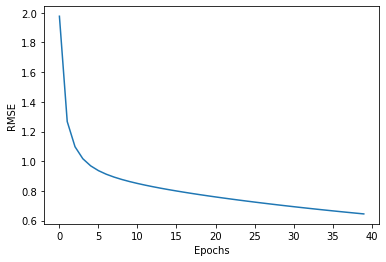
\includegraphics[width=0.5\textwidth]{./svd1.png}
\end{figure}

\begin{figure}
	\caption{RMSE plot for the second model ($\lambda=0.01$)}
	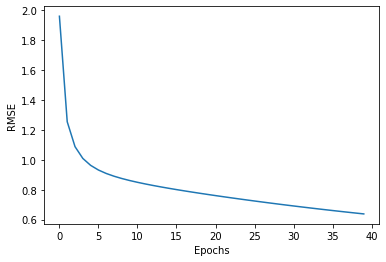
\includegraphics[width=0.5\textwidth]{./svd2.png}
\end{figure}

\begin{figure}
	\caption{RMSE plot for the third model ($k=50$)}
	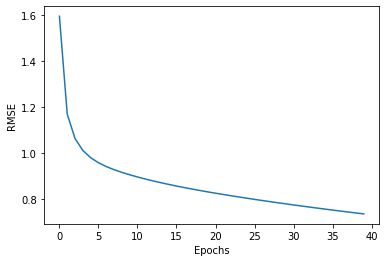
\includegraphics[width=0.5\textwidth]{./svd3.png}
\end{figure}

\begin{figure}
	\caption{RMSE plot for the fourth model ($k=10$)}
	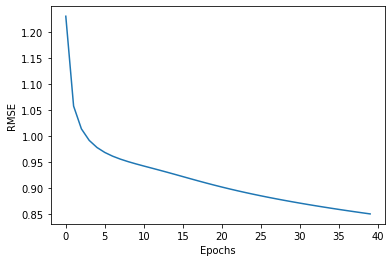
\includegraphics[width=0.5\textwidth]{./svd4.png}
\end{figure}

\begin{figure}
	\caption{RMSE plot for the fifth model ($\alpha=0.01$)}
	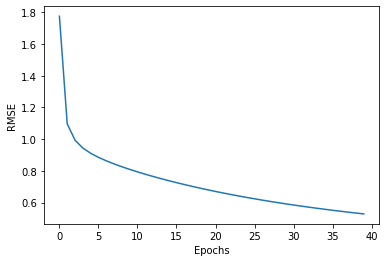
\includegraphics[width=0.5\textwidth]{./svd5.png}
\end{figure}

\subsection{Further enhancement}
We plan to split the bias terms $b_u$ and $c_i$ into terms binned by weekday or day-of-year,
i.e. $b_{u,t}, c_{i,t}$.
This allows the model to take into account effects of time on user ratings.
BigChaos~\cite{BigChaos2008} noted that this approach is helpful in offsetting long-term (probably emotional) drift of the user over time.

{\small
	\bibliographystyle{ieee_fullname}
	\bibliography{egbib}
}

\end{document}
